\section{Systems Architecture}

\subsection{System Overview Diagram}

\begin{figure}[H]
    \centering
    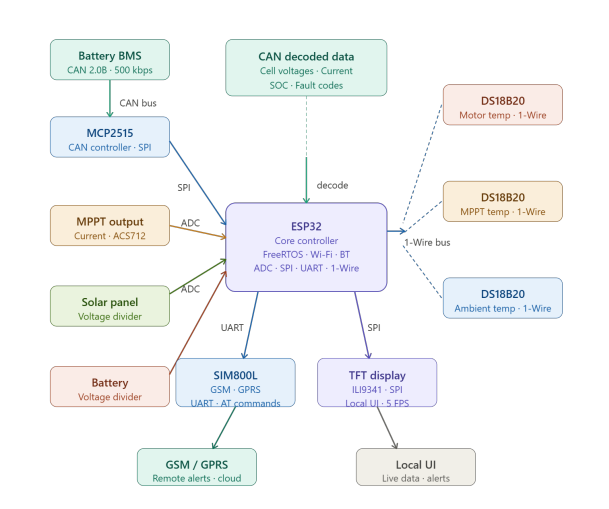
\includegraphics[width=0.85\textwidth]{images/arch-system-overview.png}
    \caption{ISS system architecture --- ESP32 core controller interfacing with the O'CELL BMS via MCP2515 CAN, three DS18B20 temperature sensors (1-Wire), ACS712 current sensors, voltage dividers, SIM800L GPRS cellular module, and local TFT display.}
    \label{fig:system-overview}
\end{figure}

The system is organised around a central ESP32 hub with five primary data flows: CAN bus communication with the BMS via MCP2515 SPI; DS18B20 digital temperature sensing on motor, MPPT, and DC/DC; ACS712/ACS758 analogue current measurement on solar panel and MPPT output; resistive divider voltage measurement at four nodes; and NPN handbrake detection. Data transmits over two parallel channels: a local Wi-Fi WebSocket server for dashboard access and a cellular GPRS/GPRS link to a cloud VPS via FastAPI into SQLite.

\subsection{Detailed System Block Diagram}

Figure~\ref{fig:diag-block} presents a detailed hardware and software block diagram of the full ISS system, from the vehicle sensors and BMS through the ISS PCB internals to the cloud backend and browser dashboard.

\begin{figure}[H]
    \centering
    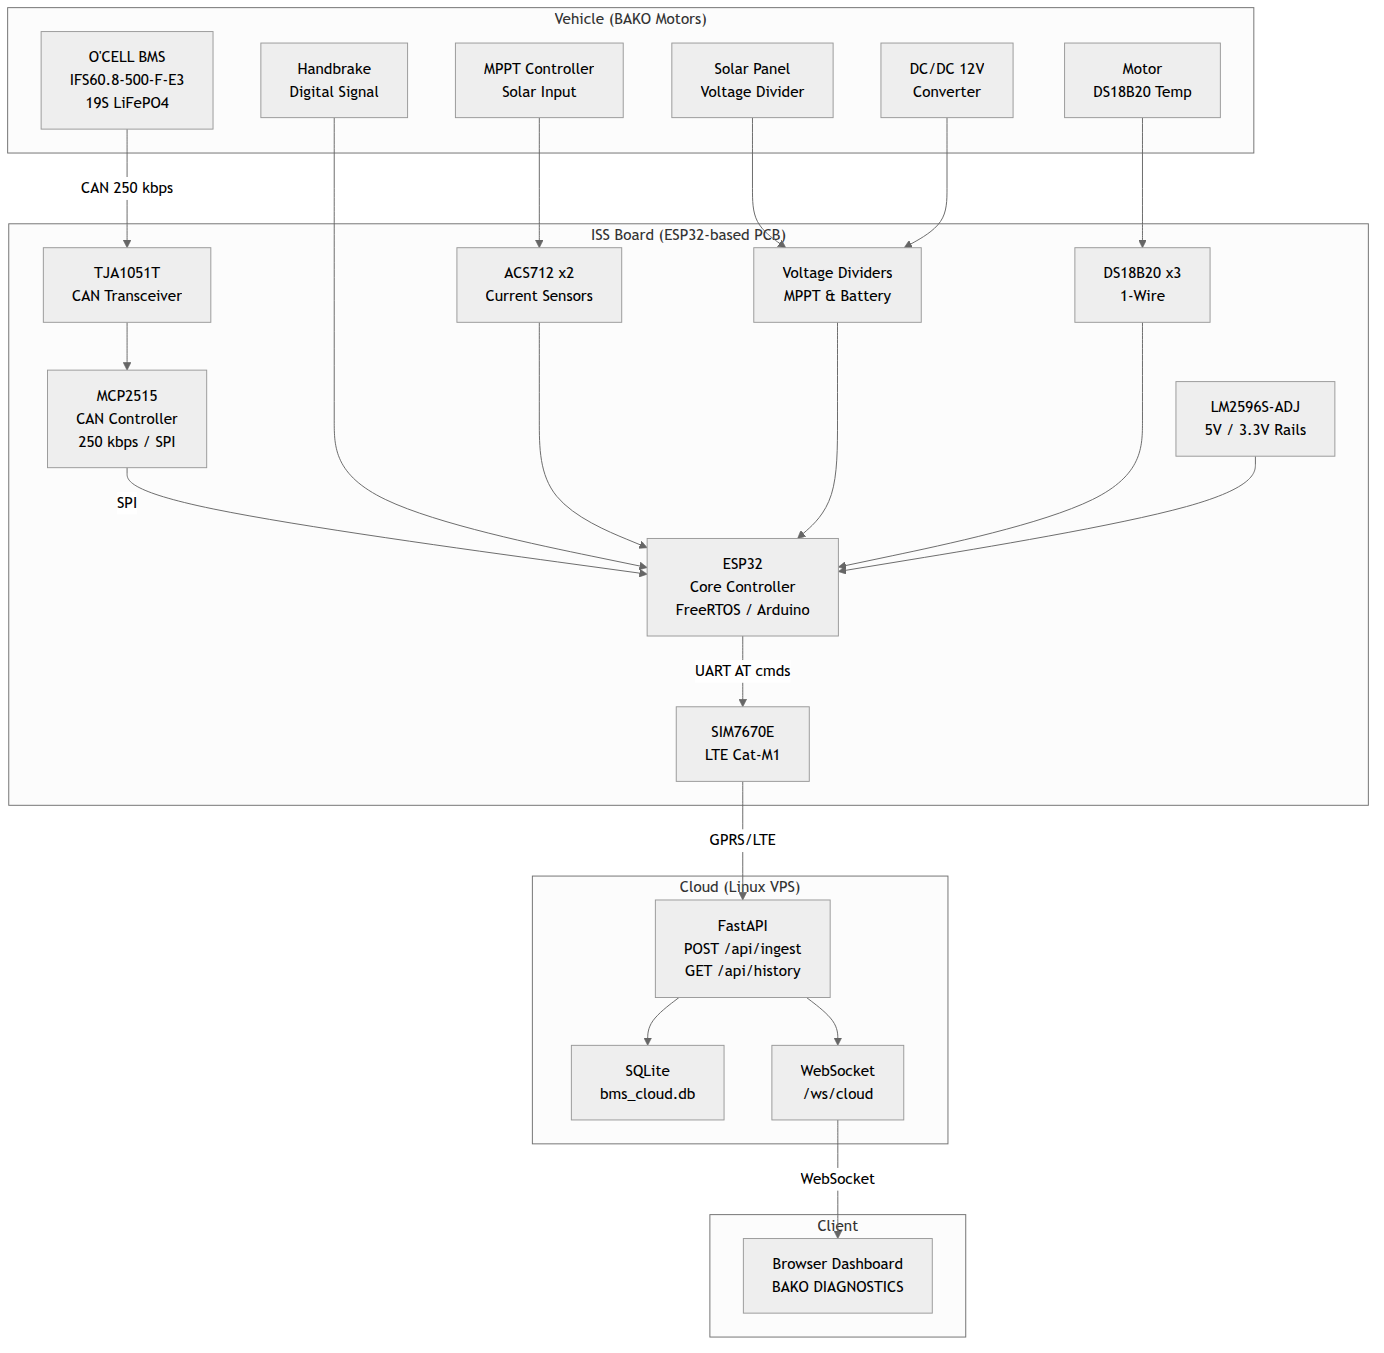
\includegraphics[width=\textwidth]{images/diag-block.png}
    \caption{Detailed ISS system block diagram showing all hardware subsystems (vehicle layer), ISS board internals (ESP32 peripherals and power regulation), cloud pipeline (FastAPI, SQLite, WebSocket), and browser client.}\label{fig:diag-block}
\end{figure}

\subsection{Electrical \& Power Systems}

The electrical and power subsystem is responsible for energy distribution, voltage regulation, and real-time monitoring of the vehicle's electrical parameters. The system integrates the battery pack, solar charging subsystem, MPPT controller, DC/DC converter, and embedded monitoring electronics.

The battery pack acts as the main energy source of the system~\cite{bakobattery} and is supervised by the Battery Management System (BMS)~\cite{ocellspec}. Communication with the BMS is established through the CAN Bus protocol~\cite{bakocan} using the MCP2515 CAN controller. The monitoring unit acquires important battery parameters such as pack voltage, current, state of charge, cell voltages, battery temperatures, and fault status information.

A solar energy subsystem is integrated to support power generation. The solar panel is connected to an MPPT (Maximum Power Point Tracking) controller, which optimises energy extraction efficiency. Current and voltage measurements are performed before and after the MPPT stage in order to evaluate charging performance and monitor power flow within the system.

The system also includes a DC/DC converter responsible for regulating voltage levels for low-power electronic components. Both input and output voltages of the converter are monitored to ensure stable operation and proper voltage regulation.

Electrical measurements are performed using ACS712 and ACS758 current sensors together with voltage sensing modules based on analogue voltage division. In addition, DS18B20 digital temperature sensors are installed on critical components such as the MPPT heatsink and DC/DC converter to supervise thermal behaviour and prevent overheating conditions.

The ESP32 microcontroller serves as the central processing and acquisition unit. It periodically collects sensor measurements and transmits the data through communication interfaces including CAN Bus, Wi-Fi, BLE, and GPRS/GPRS cellular connectivity.

\subsection{Electronic Control Units (ECUs)}

The monitoring platform integrates several Electronic Control Units (ECUs) responsible for data acquisition, communication, and system supervision. These units ensure reliable real-time monitoring of the vehicle's electrical and thermal parameters.

The main control unit of the system is the ESP32 microcontroller. It collects sensor measurements, decodes CAN Bus messages, processes data, and transmits information to the monitoring dashboard. Its integrated Wi-Fi and BLE capabilities make it suitable for embedded IoT applications.

The Battery Management System (BMS) supervises the battery pack by monitoring parameters such as voltage, current, temperature, state of charge (SOC), and fault conditions. Communication between the BMS and the ESP32 is achieved through the CAN Bus network using the MCP2515 CAN controller module.

Additional sensors are used to monitor the MPPT controller, DC/DC converter, solar panel, and motor temperature~\cite{bakomotor}. These measurements are periodically processed and transmitted by the ESP32.

During development, the ESP32 was also used as a firmware simulation platform to generate simulated sensor data and CAN frames. This allowed testing the dashboard and communication interfaces without continuously connecting the system to the vehicle, simplifying debugging and software validation.

Overall, the ECU architecture provides efficient monitoring, communication, and diagnostic capabilities for the vehicle monitoring platform.

\subsection{Embedded Software Architecture}
\label{sec:embedded-sw-arch}

The embedded software running on the ESP32 microcontroller is structured as a \textbf{single-threaded, cooperative loop} built on the Arduino framework. This architecture was chosen for its simplicity and determinism: all BMS-related tasks execute sequentially on one core, eliminating the need for inter-task synchronization.

The software is divided into five logical layers, shown in Figure~\ref{fig:sw-layers}:

\begin{figure}[H]
    \centering
    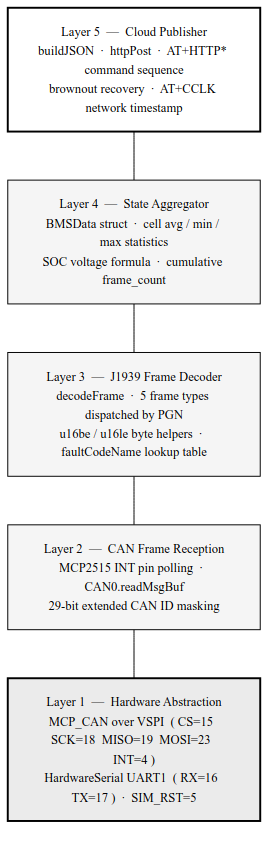
\includegraphics[width=0.45\textwidth]{images/sw-layers.png}
    \caption{ESP32 embedded software layer diagram}
    \label{fig:sw-layers}
\end{figure}

\begin{description}
    \item[Hardware Abstraction Layer (HAL)]
    Provides direct access to the MCP2515 via SPI (\texttt{mcp\_can} library) and to the SIM800L via HardwareSerial UART1. Pin assignments and bus parameters (CS, INT, baud rate, crystal frequency) are defined as constants and isolated from the application logic.

    \item[CAN Frame Reception]
    The MCP2515 asserts the \texttt{INT} line (GPIO 4) when a frame is placed in its receive buffer. The main loop polls this line and calls \texttt{CAN0.readMsgBuf()} to drain all pending frames. Extended CAN IDs are masked from the 29-bit field before processing.

    \item[J1939 Decoder]
    The \texttt{decodeFrame()} function dispatches each received frame by inspecting the \texttt{FUNC} byte of the CAN ID (bits 23--16). It handles five frame types (cell voltages, temperatures, BMS Basic 1 \& 2, charging request) and writes decoded values into the \texttt{BMSData} struct.

    \item[State Aggregator]
    The \texttt{BMSData} struct accumulates all decoded fields and maintains derived statistics (cell average, min, max, voltage-based SOC). The struct is updated in place and always holds the most recent complete state of the battery.

    \item[Cloud Publisher]
    Every 5 seconds, \texttt{buildJSON()} serializes \texttt{BMSData} into a JSON document using the ArduinoJson library, and \texttt{httpPost()} delivers it to the VPS via the SIM800L AT+HTTP* command set.
\end{description}

\subsubsection{Key Design Decisions}

\textbf{No explicit RTOS task management.} A FreeRTOS multi-task structure was considered but rejected because the single-responsibility loop handles all timing requirements naturally: CAN frames arrive at 100--500 ms intervals, and the publish cycle runs every 5 seconds. Adding preemptive scheduling would have introduced stack management and mutex overhead without any functional benefit.

\textbf{CAN drain during HTTP wait.} The \texttt{AT+HTTPACTION} response can take up to 30 seconds over a cellular link. To prevent the MCP2515 receive buffer (6 frames deep) from overflowing during this window, the HTTP wait loop polls the CAN \texttt{INT} pin and drains frames continuously, calling \texttt{decodeFrame()} in-place. This ensures the \texttt{BMSData} struct is fully up-to-date when the next publish cycle begins.

\textbf{HardwareSerial over SoftwareSerial.} SoftwareSerial operates via bit-banging and is sensitive to interrupt latency. The SIM800L produces multi-line AT response bursts that SoftwareSerial occasionally drops bytes from at 9600 baud on a loaded core. HardwareSerial UART1 uses dedicated silicon and a hardware FIFO, making it robust under all operating conditions.

% ─────────────────────────────────────────────────────────────────────────────
\subsection{Cloud \& Connectivity Architecture}
\label{sec:cloud-arch}

The cloud and connectivity architecture connects the on-vehicle ESP32 to a remote browser with minimal intermediaries. The full pipeline is shown in Figure~\ref{fig:cloud-arch}.

\begin{figure}[H]
    \centering
    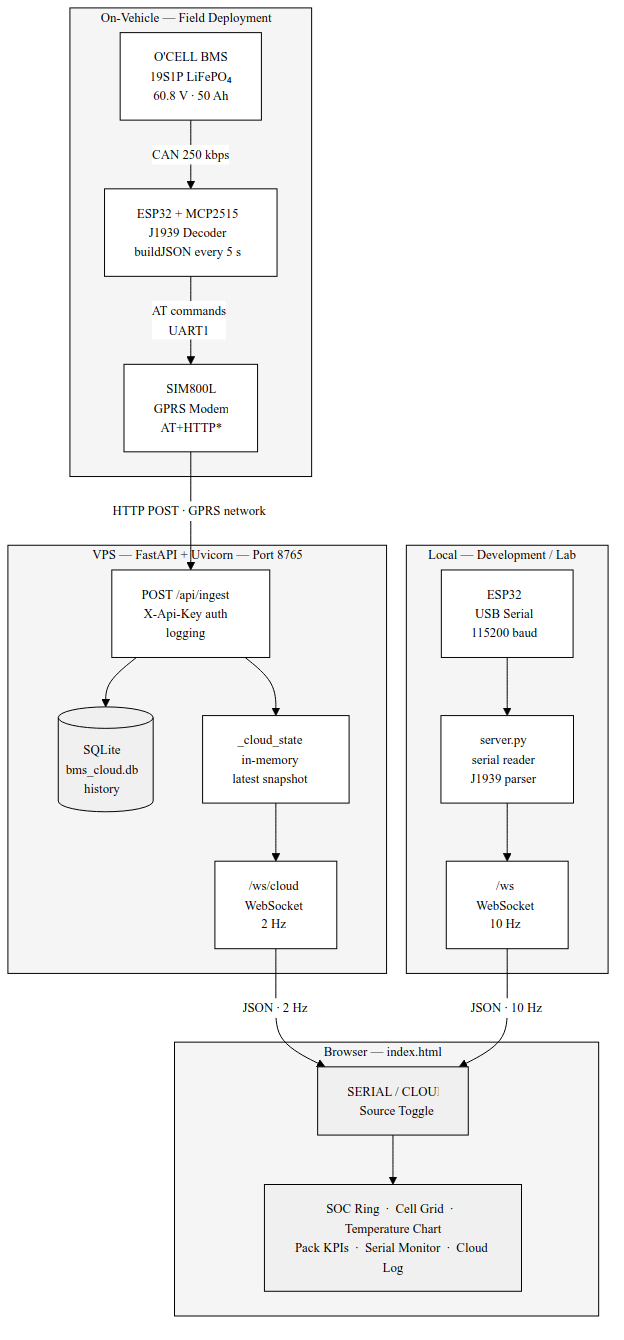
\includegraphics[width=0.5\textwidth]{images/cloud-arch.png}
    \caption{End-to-end cloud connectivity architecture}
    \label{fig:cloud-arch}
\end{figure}

\subsubsection{Component Roles}

\begin{description}
    \item[ESP32 + MCP2515 (On-vehicle edge node)]
    Reads and decodes SAE J1939 CAN frames from the BMS at up to 10 frames per second, aggregates them into a snapshot, and transmits one JSON document to the VPS every 5 seconds.

    \item[SIM800L GPRS Module]
    Provides wide-area cellular connectivity over GPRS Cat-M1 using the carrier network. Communicates with the ESP32 via AT commands over UART. Handles TCP/IP, HTTP, and DNS entirely on-chip using the AT+HTTP* service, so the ESP32 only needs to manage the AT command dialogue. The SIM800L-CORE footprint is used as the PCB layout placeholder; the physically populated component is the SIM800L.

    \item[VPS Backend (FastAPI + Uvicorn)]
    Acts as the single ingestion point and real-time relay for all cloud data. Receives POST requests from the ESP32, stores them to SQLite for persistence, and maintains an in-memory state that is pushed to connected browser clients via WebSocket at 2 Hz. The server also handles the SERIAL mode WebSocket, allowing the same dashboard to be used with a direct USB connection.

    \item[SQLite Database]
    Provides persistent local storage for all received snapshots. Enables historical data retrieval via the \texttt{/api/history} endpoint without any external database service.

    \item[Browser Dashboard]
    A single-page web application that renders live battery data received over WebSocket. Supports SERIAL mode (direct USB, 10 Hz) and CLOUD mode (VPS relay, 2 Hz). Auto-reconnects on network interruption.
\end{description}

\subsubsection{Data Flow Summary}

\begin{enumerate}
    \item O'CELL BMS $\rightarrow$ CAN bus (250 kbps, SAE J1939)
    \item ESP32 + MCP2515 $\rightarrow$ decode all frames $\rightarrow$ \texttt{BMSData} struct
    \item ESP32 $\rightarrow$ \texttt{buildJSON()} $\rightarrow$ JSON document
    \item ESP32 $\rightarrow$ SIM800L AT+HTTPACTION=1 $\rightarrow$ \texttt{POST /api/ingest} (HTTP, GPRS)
    \item VPS server $\rightarrow$ validate API key $\rightarrow$ SQLite insert + in-memory update
    \item VPS server $\rightarrow$ \texttt{/ws/cloud} WebSocket push every 2 s
    \item Browser $\rightarrow$ render panels (SOC, cells, temperatures, faults, cloud log)
\end{enumerate}

\subsubsection{Dual-Mode Operation}

A key architectural feature is that the dashboard supports two independent data sources via the same frontend interface. In \textbf{SERIAL mode}, the backend reads raw CAN log lines from the ESP32 USB serial port, decodes them through its own Python J1939 parser (\texttt{BMSState.decode()}), and pushes the result at 10 Hz. In \textbf{CLOUD mode}, the backend serves the latest snapshot received from the ESP32 over GPRS.

This dual-mode design provides two practical benefits:
\begin{itemize}
    \item During development and testing, the system can be operated entirely over USB without requiring a SIM card or GPRS connection.
    \item In the field, the dashboard can be opened from any web browser pointed at the VPS IP address, with no local software to install.
\end{itemize}

\subsection{3D Mechanical Architecture}

The 3D mechanical architecture of the ISS board is described in Chapter~7 (Mechanical Design). The two-layer PCB is dimensioned to fit within a standard DIN-rail enclosure, with all external connectors (CAN bus, sensor headers, power input) placed along the board perimeter for clean harness routing. A 3D render of the board is shown in Figure~\ref{fig:pcb-3d}.

\subsection{Safety \& Redundancy Design}

\subsubsection*{Hardware Protection}

Reverse polarity protection is implemented at the main power input using diode D6, which prevents damage to all downstream circuitry in the event of an incorrect supply connection. Overcurrent protection is provided by fuses F1, F2, and F3, placed on the main power rail and the sensor supply lines respectively, limiting fault currents before they can damage components. Zener diodes D3, D4, and D7 provide ESD and overvoltage clamping on the CAN bus lines, protecting the MCP2515 and TJA1051T transceiver from voltage spikes induced by the vehicle's electrical environment.

\subsubsection*{Software Redundancy}

A hardware watchdog timer ensures automatic recovery from firmware hangs by resetting the ESP32 microcontroller without requiring manual intervention. The MCP2515 CAN error counter is monitored continuously; if the error count exceeds the bus-off threshold --- which can occur after a transient disconnection or excessive noise on the CAN bus --- the driver automatically re-initialises the controller and resumes normal frame reception. All ADC input readings are subject to sanity-check bounds validation before being stored in the telemetry structure, discarding implausible values caused by transient noise or sensor disconnection. Threshold violation alerts for over-temperature, over-voltage, and over-current conditions are transmitted via SMS through the SIM800L module, enabling remote notification of critical fault events without requiring an active internet connection.
